\chapter{HeROsim : Élaborer et évaluer des politiques d'orchestration serverless pour le cloud privé}
\label{chapter:herosim}

% TODO: nouvelles références à intégrer~\cite{bambrikSurveyCloudComputing2020, byrneReviewCloudComputing2017}

% TODO: màj bibtex (références raccourcies pour IEEE IC)

\section{Introduction}
\label{section:herosim-introduction}

Les deux chapitres précédents ont abordé un ensemble de défis qui doivent être relevés par les fournisseurs de services qui souhaitent déployer des applications sur une plateforme serverless optimisée pour la \gls{QoS} et économe en énergie. Le chapitre~\ref{chapter:herofake} traite en particulier de la surcharge de latence causée par l'allocation dynamique du matériel pour les nouvelles instances de fonction, appelée délai de démarrage à froid~\cite{vahidiniaColdStartServerless2020}. Un autre problème récurrent, introduit dans le chapitre~\ref{chapter:herocache}, est celui de la prise en compte de la localité des données~\cite{yuFollowingDataNot} par la plateforme pour éviter une dégradation considérable des performances, en particulier dans le cas d'applications conçues comme des chaînes de fonctions qui communiquent entre elles.

Pour surmonter de tels défis, nous avons conçu des politiques d'orchestration qui guident les décisions d'allocation de ressources et d'ordonnancement de requêtes, dans le but de minimiser les coûts, selon des objectifs d'optimisation définis par le fournisseur de services. Il est nécessaire d'évaluer la pertinence de ces politiques dans divers cas d'utilisation ; différentes mesures peuvent être utiles pour cette évaluation, par exemple la durée totale de complétion pour un scénario donné, le temps de réponse des fonctions, la consommation d'énergie dynamique et statique dans la plateforme, etc.

\boitemagique{Question 3 (\textbf{QR3})}{
    Du point de vue d'un fournisseur de services pour le cloud, comment évaluer et comparer l'impact sur la qualité de service de différentes politiques d'allocation de ressources et d'ordonnancement de tâches dans le modèle serverless ?
}

Il y a deux façons possibles d'évaluer si les politiques que nous concevons ont un impact positif sur ces mesures : la simulation (estimation) ou la mise en œuvre (mesure). Ces deux approches présentent un compromis entre temps, coût et précision ; choisir la simulation plutôt que la mise en œuvre permet de parcourir l'espace du problème en itérant rapidement sur des solutions possibles. En particulier, la modélisation à événements discrets nous permet d'explorer des solutions en représentant les différents composants de la plateforme avec des processus qui modélisent l'état du système et son évolution dans le temps.

L'orchestration est un processus dynamique : chaque décision crée un nouvel état pour le système, ce qui conduit à une explosion combinatoire. De plus, les plateformes serverless sont des logiciels génériques qui exposent de nombreux paramètres sur lesquels le fournisseur peut agir. Ces paramètres peuvent avoir un impact sur la latence des requêtes des utilisateurs, le débit de la plateforme, l'utilisation des ressources et la consommation d'énergie de l'infrastructure. Comme il est coûteux d'expérimenter en production, nous soutenons que les outils de simulation sont essentiels pour les fournisseurs de cloud serverless privé qui cherchent à optimiser ces mesures de qualité de service en fonction de leurs propres objectifs.

Les outils de simulation des politiques d'orchestration dans le cloud serverless privé doivent permettre de tracer les événements d'allocation des ressources et de placement des tâches à la \textbf{granularité la plus fine}, afin de comprendre l'impact des politiques sur les métriques de performance. Pour représenter des cas d'utilisation réalistes, le logiciel doit offrir la possibilité de modéliser des applications qui présentent des \textbf{dépendances de données et temporelles} entre les exécutions de tâches. En outre, le simulateur doit prendre en charge l'hétérogénéité globale dans le cloud : d'une part, les centres de données sont constitués de divers matériels présentant différents niveaux de coût et de performance ; d'autre part, il existe un large éventail d'utilisateurs ayant des exigences différentes en matière de qualité de service. Enfin, le simulateur devrait pouvoir \textbf{rejouer les traces d'exécution} pour différentes politiques d'orchestration et \textbf{comparer les résultats} en termes de métriques de qualité de service pour chaque politique évaluée.

\begin{table*}[!ht]
    \centering
    \caption{État de l'art des outils de simulation pour l'orchestration des ressources et des charges de travail dans le cloud.}
    \resizebox{\linewidth}{!}{
        \begin{tabular}{lYYYYYYYYY}
        \toprule
        & Serverless & Déploiements & Chaînes de fonctions & Hétérogénéité matérielle & \gls{QoS} par requête & Énergie & Visualisation \\
        \cmidrule(lr){2-2}\cmidrule(lr){3-3}\cmidrule(lr){4-4}\cmidrule(lr){5-5}\cmidrule(lr){6-6}\cmidrule(lr){7-7}\cmidrule(lr){8-8}
        CloudSim~\cite{calheiros_cloudsim_2011} & \xmark & Public, privé, hybride & \xmark & \cmark & \xmark & \cmark & \xmark \\
        CloudSimSC~\cite{mampage_cloudsimsc_2023} & \cmark & Public, privé, hybride & \xmark & \cmark & \xmark & \cmark & \xmark \\
        CloudAnalyst~\cite{wickremasinghe_cloudanalyst_2010} & \xmark & Public, privé, hybride & \xmark & \cmark & \xmark & \cmark & \cmark \\        DFaaSCloud~\cite{jeonCloudSimExtensionSimulatingDistributed2019} & \cmark & Hybride multi-strates & \xmark & \xmark & \cmark & \xmark & \cmark \\
        ElasticSim~\cite{cai_elasticsim_2017} & \xmark & Public & \cmark & \xmark & \xmark & \xmark & \cmark \\
        GridSim~\cite{buyyaGridSimToolkitModeling2002} & \xmark & Grille & \xmark & \cmark & \cmark & \xmark & \cmark \\
        iCanCloud~\cite{nunez_icancloud_2012} & \xmark & Public & \xmark & \xmark & \xmark & \xmark & \cmark \\
        iFogSim2~\cite{mahmudIFogSim2ExtendedIFogSim2021} & \xmark & Edge, Fog & \xmark & \cmark & \xmark & \cmark & \xmark \\
        OpenDC 2.0~\cite{mastenbroekOpenDCConvenientModeling2021} & \cmark & Public, privé, hybride & \cmark & \cmark & \xmark & \cmark & \cmark \\
        SimFaaS~\cite{mahmoudiSimFaaSPerformanceSimulator2021} & \cmark & Public & \xmark & \xmark & \xmark & \cmark & \cmark \\
        \textbf{HeROsim} & \cmark & Privé & \cmark & \cmark & \cmark & \cmark & \cmark \\
        \bottomrule
        \end{tabular}
    }
    \label{table:herosim-sota}
\end{table*}

Des travaux antérieurs ont proposé différents outils de simulation intéressants pour le cloud, que nous présentons au regard de leurs caractéristiques dans le tableau~\ref{table:herosim-sota} ; le chapitre~\ref{chapter:sota} donne plus de détails en section~\ref{section:sota-herosim}. Certains de ces travaux ne ciblent pas le paradigme serverless~\cite{calheiros_cloudsim_2011, wickremasinghe_cloudanalyst_2010, cai_elasticsim_2017, buyyaGridSimToolkitModeling2002, nunez_icancloud_2012, mahmudIFogSim2ExtendedIFogSim2021}. Parmi les simulateurs serverless, certains se concentrent sur les offres de cloud public~\cite{nunez_icancloud_2012, mahmoudiSimFaaSPerformanceSimulator2021}, principalement pour permettre de concevoir des stratégies hybrides où une partie des charges de travail est déléguée à un cloud public, moins coûteux. Pour le cloud privé, certains simulateurs ne prennent pas en compte la consommation d'énergie~\cite{jeonCloudSimExtensionSimulatingDistributed2019, cai_elasticsim_2017, buyyaGridSimToolkitModeling2002, nunez_icancloud_2012} ; d'autres considèrent une infrastructure homogène~\cite{jeonCloudSimExtensionSimulatingDistributed2019, nunez_icancloud_2012, mahmoudiSimFaaSPerformanceSimulator2021}. La plupart des simulateurs de plateformes serverless ne permettent pas de modéliser des applications composées de multiples fonctions avec des dépendances de données~\cite{calheiros_cloudsim_2011, mampage_cloudsimsc_2023, wickremasinghe_cloudanalyst_2010, jeonCloudSimExtensionSimulatingDistributed2019, buyyaGridSimToolkitModeling2002, nunez_icancloud_2012, mahmudIFogSim2ExtendedIFogSim2021}. Dans certaines études, la qualité de service ne peut pas être spécifiée à la granularité d'une requête utilisateur~\cite{calheiros_cloudsim_2011, mampage_cloudsimsc_2023, wickremasinghe_cloudanalyst_2010, cai_elasticsim_2017, nunez_icancloud_2012, mahmudIFogSim2ExtendedIFogSim2021, mastenbroekOpenDCConvenientModeling2021, mahmoudiSimFaaSPerformanceSimulator2021}.

Pour remédier à ces limitations, nous proposons \textbf{HeROsim}~\footnote{\href{https://github.com/b-com/HeROsim}{https://github.com/b-com/HeROsim}} (pour \textbf{He}terogeneous \textbf{R}esources \textbf{O}rchestration \textbf{sim}ulator), un simulateur pour le cloud privé serverless, libre et open source (licence Apache 2.0~\footnote{\href{https://www.apache.org/licenses/LICENSE-2.0}{https://www.apache.org/licenses/LICENSE-2.0}}), présentant les caractéristiques suivantes :

\begin{itemize}
    \item Description fine des applications serverless sur du matériel hétérogène : les fonctions sont définies selon un ensemble de métadonnées sur leurs performances, flux de données, besoins en mémoire, consommation d'énergie ;
    \item Allocation dynamique des ressources matérielles et placement des requêtes utilisateur compatibles avec la qualité de service : HeROsim offre des points d'entrée aux utilisateurs pour mettre en œuvre leurs propres politiques de sélection des ressources, à la granularité d'une requête ;
    \item Évaluation des politiques d'orchestration en fonction de paramètres de qualité de service : HeROsim permet de comparer les résultats de différentes stratégies en termes de métriques couramment utilisées pour mesurer la qualité de service, tels que la latence et l'énergie.
\end{itemize}

La conception du logiciel suit l'architecture de référence des orchestrateurs de l'état de l'art tels que Google Knative~\footnote{\href{https://knative.dev}{https://knative.dev}} ou Apache OpenWhisk~\footnote{\href{https://openwhisk.apache.org}{https://openwhisk.apache.org}}. Ces orchestrateurs se composent de deux modules principaux, comme montré dans la figure~\ref{figure:herosim-platform} :

\begin{itemize}
    \item Un \textbf{autoscaler} qui détermine comment mettre à l'échelle automatiquement et de manière réactive les ressources matérielles disponibles dans l'infrastructure, en adéquation avec la charge sur les applications ;
    \item Un \textbf{ordonnanceur} qui détermine sur quelle réplique mettre en file d'attente les requêtes utilisateur pour une fonction donnée, étant données des exigences de qualité de service définies au niveau des requêtes.
\end{itemize}

Ce chapitre est organisé comme suit : la section~\ref{section:herosim-overview} donne un aperçu du fonctionnement d'une plateforme serverless ; la section~\ref{section:herosim-herosim} détaille la conception de HeROsim ; la section~\ref{section:herosim-case-study} montre comment HeROsim peut être exploité à travers deux cas d'utilisation tirés de nos publications ; enfin, nous concluons par les limites de la contribution et quelques perspectives pour de futurs travaux en section~\ref{section:herosim-conclusion}.
% nous discutons ensuite dans la section~\ref{section:herosim-sota} des travaux de l'état de l'art ; 

\section{Présentation générale de la plateforme simulée}
\label{section:herosim-overview}

\begin{figure*}[!ht]
    \centering
    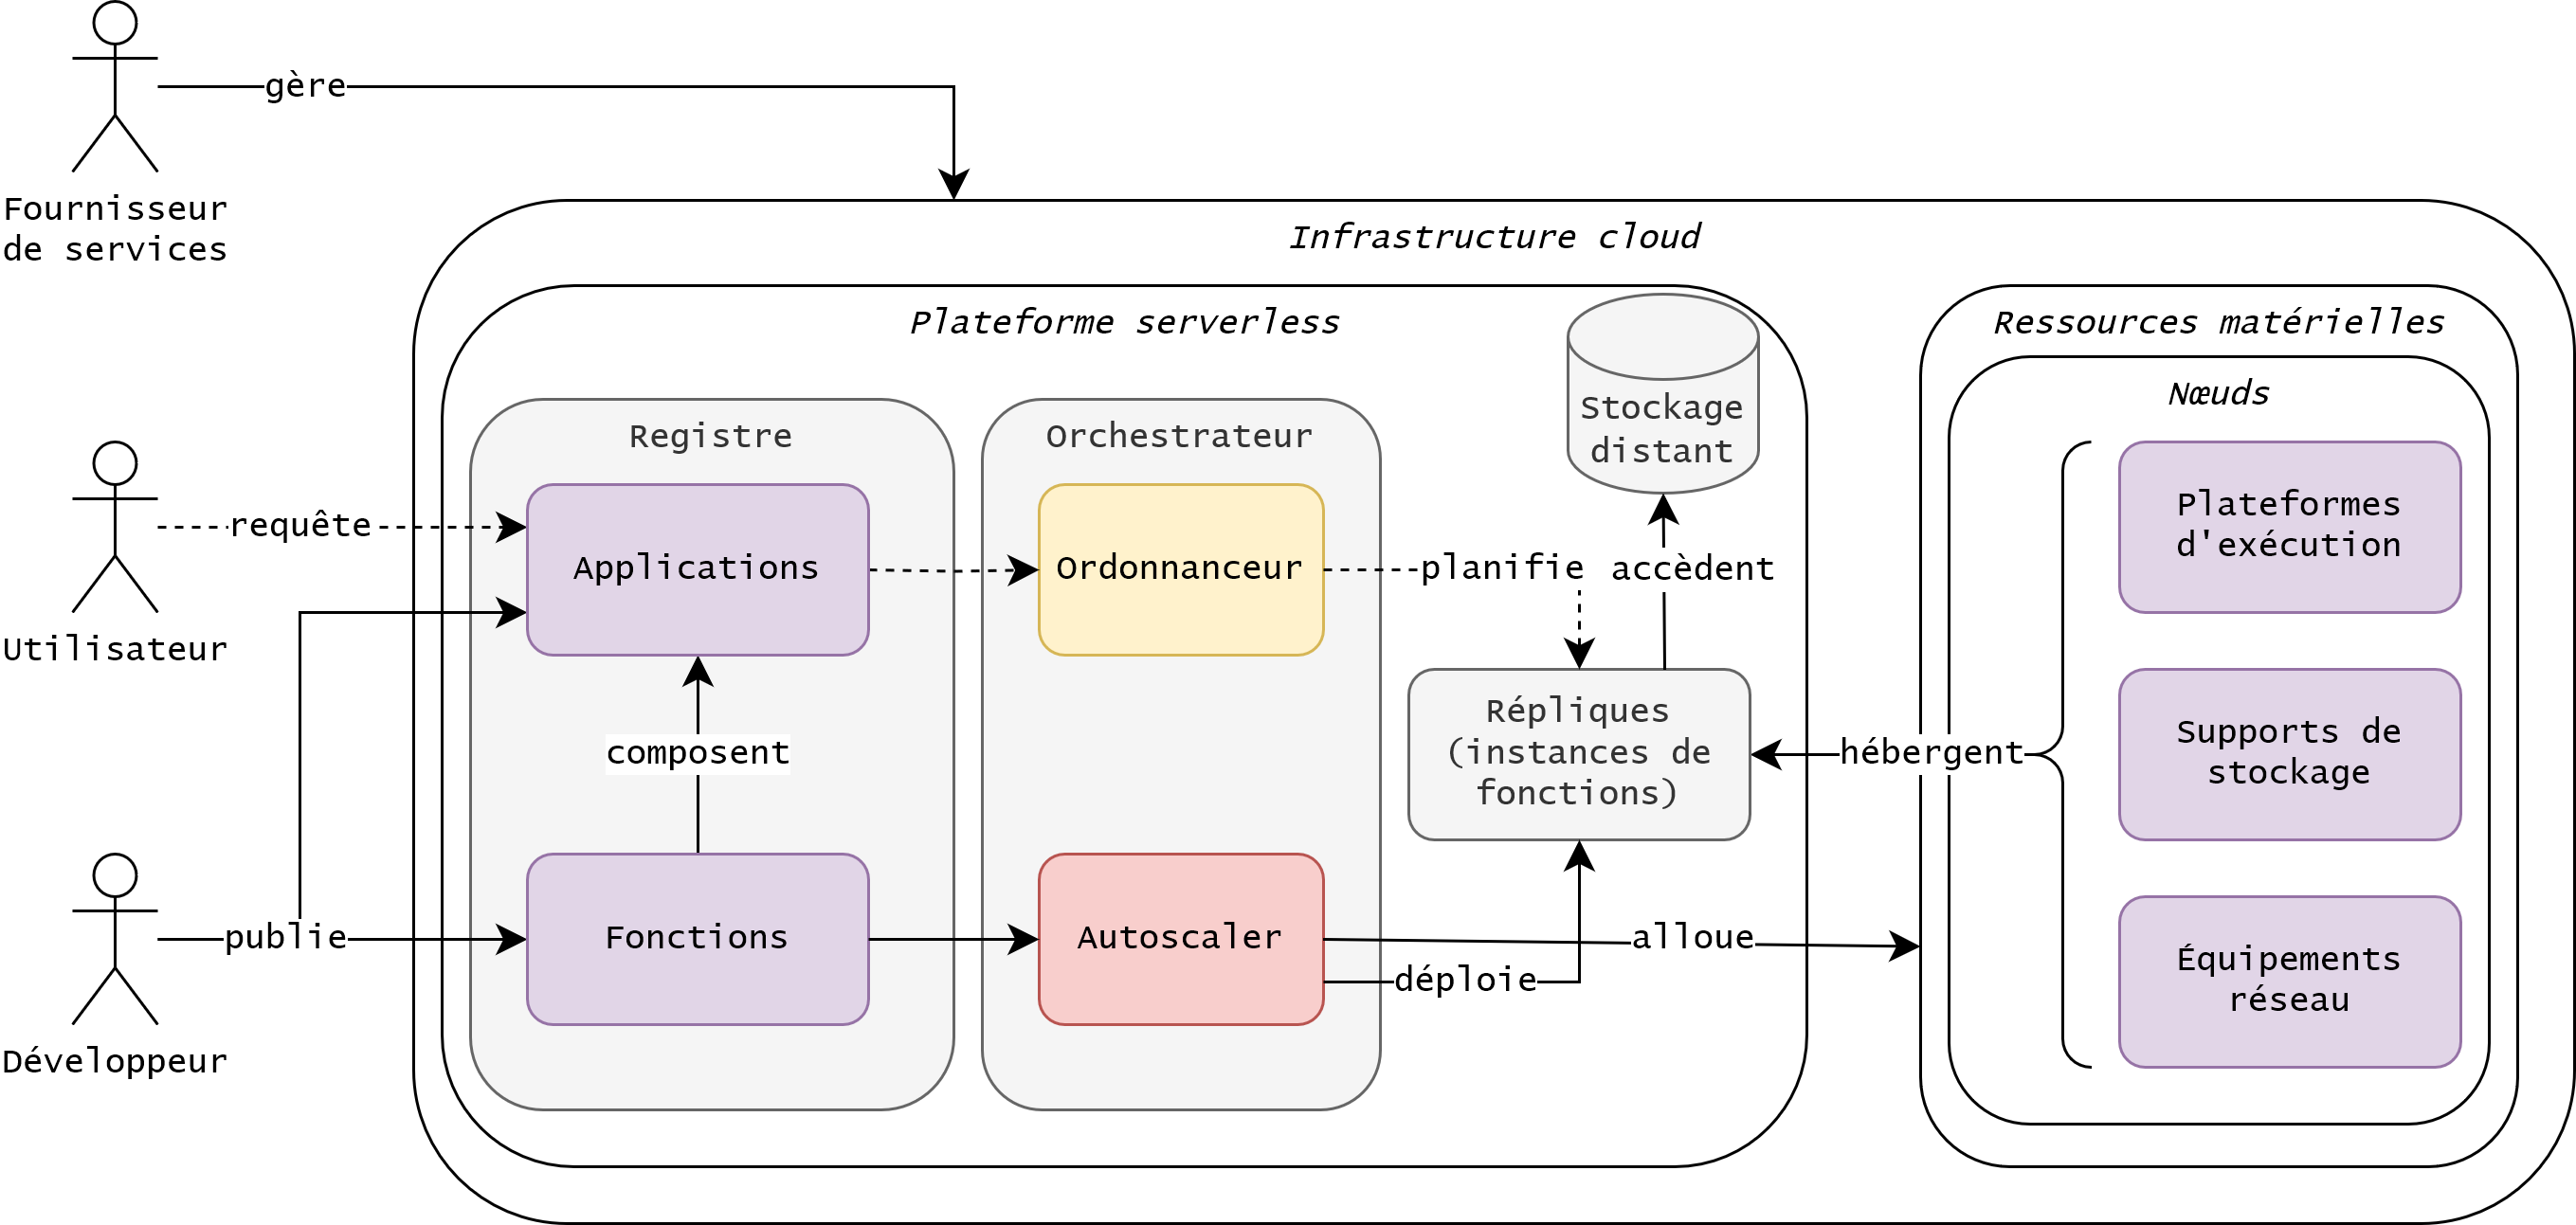
\includegraphics[width=0.9\textwidth]{6_Chapitre6/figures/platform-complete.png}
    \caption{Vue de haut niveau d'une plateforme serverless, telle que modélisée dans HeROsim. L'autoscaler alloue des ressources matérielles pour les répliques de fonctions ; tandis que l'ordonnanceur place les requêtes utilisateur en file d'attente sur ces répliques.}
\label{figure:herosim-platform}
\end{figure*}

Dans les modèles de service traditionnels pour le cloud (voir chapitre~\ref{chapter:context}), les clients réservent généralement des ressources auprès d'un fournisseur de services. Il s'agit d'un sous-ensemble virtualisé de ressources matérielles hétérogènes disponibles sur des serveurs appelés nœuds. Une fois la réservation effectuée, la plateforme cloud offre un accès à distance aux clients, qui sont responsables du déploiement de leurs applications, et facturés en fonction de la quantité de ressources qu'ils ont réservée~\cite{Lannurien2023}.

Dans le paradigme serverless, les clients commencent par mettre en ligne le code de leur application dans un registre du côté du fournisseur, comme illustré par la figure~\ref{figure:herosim-platform}. Le fournisseur alloue des ressources qui sont automatiquement mises à l'échelle en fonction de la charge sur l'application. Pour que ce mécanisme fonctionne, les applications sont divisées en petites unités d'exécution appelées \textbf{fonctions}. Ces fonctions sont dites sans état : si elles produisent des données de sortie, celles-ci doivent être conservées dans un stockage persistant~\cite{yuFollowingDataNot}.

Dans les modèles de service traditionnels, les ressources sont mises à l'échelle sur deux dimensions : horizontalement (nouvelles instances d'application créées sur d'autres nœuds) et verticalement (ressources supplémentaires allouées aux instances existantes). Dans les plateformes serverless, les ressources sont mises à l'échelle horizontalement : les variations de charge sur les applications sont absorbées par l'ajout de nouvelles instances des fonctions, appelées \textbf{répliques}, et par leur suppression lorsqu'elles ne sont plus nécessaires. Une réplique peut être créée pour chaque requête utilisateur, ou réutilisée pour plusieurs requêtes. On peut considérer les répliques de fonctions comme des files d'attente de requêtes ayant des capacités différentes.

Ces répliques sont créées par l'\textbf{autoscaler}. Pour gérer le nombre de répliques déployées pour chaque fonction, il existe trois stratégies principales : une stratégie par requête, une stratégie par niveau de concurrence, et une stratégie par métriques~\cite{mahmoudiSimFaaSPerformanceSimulator2021}. Dans la première stratégie, chaque requête entrante est traitée par une réplique inactive. Si aucune réplique inactive n'est disponible, une nouvelle instance de la fonction est créée ; le nombre de répliques pour chaque fonction dépend donc directement du nombre de requêtes à traiter à un instant donné. Dans l'autoscaling basé sur la concurrence, chaque réplique peut mettre en file d'attente plusieurs requêtes utilisateur pour les traiter séquentiellement ; le nombre de répliques dépend du nombre de requêtes en attente pour chaque fonction, rapporté à un seuil de concurrence prédéfini~\cite{herofake}. Dans l'autoscaling basé sur les métriques, le nombre de répliques déployées dépend de divers objectifs, tels que le taux de requêtes par seconde (\gls{RPS}) à atteindre ; pour ce faire, l'autoscaler doit avoir une vue sur les performances et l'état global du système.

Les répliques peuvent se trouver dans trois états différents : initialisation, exécution et inactivité~\cite{SchleierSmith2021WhatSC}. Lorsqu'une réplique de fonction vient d'être créée, elle est en état d'initialisation : la plateforme instancie son environnement d'exécution, extrait le code de la fonction depuis un registre distant et le met éventuellement en cache sur le nœud de déploiement, puis commence à exécuter la fonction. Lorsque la réplique traite les requêtes utilisateur, elle est en état d'exécution. Dans le cas contraire, la réplique est inactive et peut être supprimée, ou gardée en vie dans un état prêt à traiter d'éventuelles futures requêtes. Lorsqu'une réplique est supprimée, les ressources matérielles qui lui avaient été allouées sont libérées : la création d'une nouvelle réplique pour traiter une requête utilisateur entrante entraîne un \textbf{démarrage à froid}. Les orchestrateurs adoptent diverses politiques pour atténuer ce problème, allant de l'application d'une période de maintien en vie sur les répliques de fonctions pour éviter de les détruire trop tôt, à l'allocation proactive de ressources pour initialiser des répliques en avance de phase. L'orchestrateur fait alors un compromis entre utilisation des ressources et performances.

Enfin, les requêtes utilisateur sont attribuées aux répliques de fonctions disponibles par l'\textbf{ordonnanceur} qui met en œuvre différentes stratégies : par exemple, \gls{AWS} Lambda\footnote{\href{https://aws.amazon.com/en/lambda/}{https://aws.amazon.com/en/lambda/}} utilise un algorithme de \textit{bin-packing}, tandis qu'une plateforme open source telle que Knative met en œuvre une politique d'équilibrage de la charge~\cite{Lannurien2023}. Ces stratégies ont des résultats différents en ce qui concerne l'utilisation des ressources et la qualité de service, mais il peut être difficile de prédire dans quelle mesure elles auront un impact sur les charges de travail avant de pouvoir l'observer en production.

\section{Choix de conception}
\label{section:herosim-herosim}

Cette section présente les choix de conception et les hypothèses formulées pour le développement de HeROsim.

\begin{figure}[!ht]
    \centering
    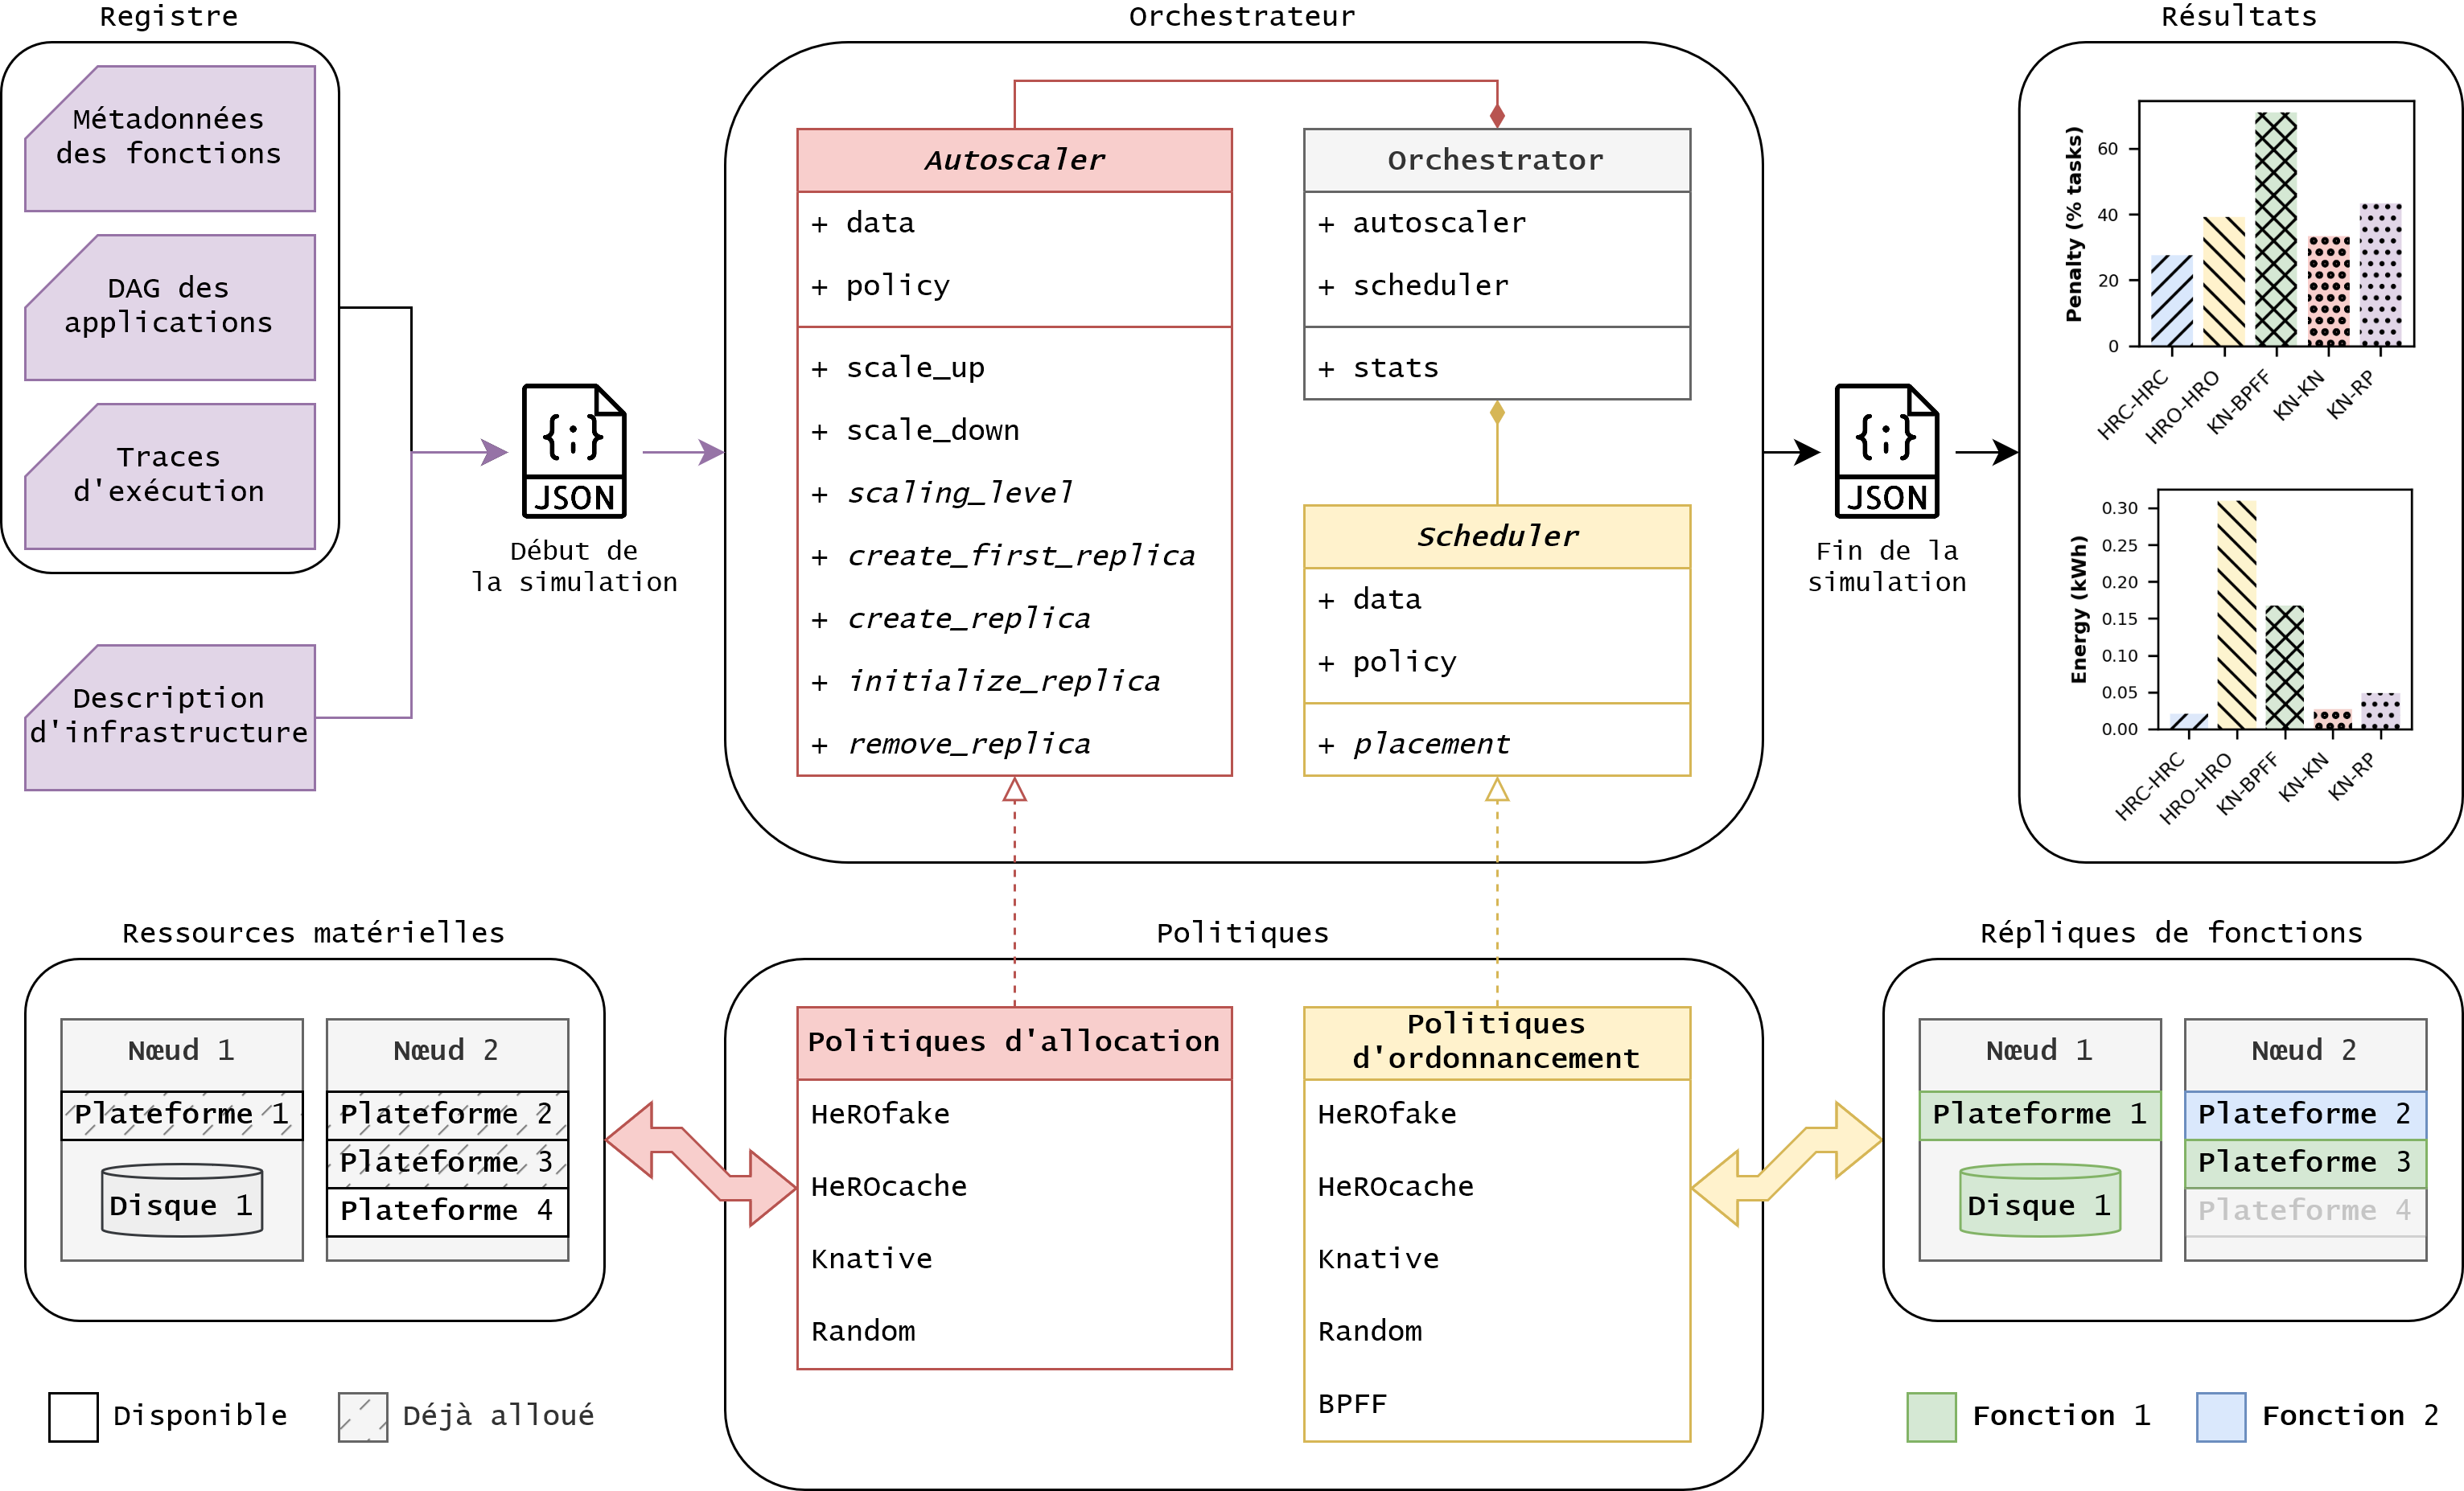
\includegraphics[width=0.9\textwidth]{6_Chapitre6/figures/software-architecture.png}
    \caption{Vue de haut niveau de l'architecture logicielle du simulateur.}
\label{figure:herosim-software-architecture}
\end{figure}

HeROsim utilise la bibliothèque SimPy~\footnote{\href{https://simpy.readthedocs.io}{https://simpy.readthedocs.io}} comme moteur de simulation à événements discrets. Cette bibliothèque est disponible sous licence libre (\textit{MIT}) ; elle est largement documentée et utilisée dans la recherche~\cite{matloffIntroductionDiscreteEventSimulation, zinovievDiscreteEventSimulation2024a}. Notre simulateur fournit trois classes de base, comme montré dans la figure~\ref{figure:herosim-software-architecture} -- \texttt{Orchestrator}, \texttt{Autoscaler} et \texttt{Scheduler} -- destinées à être sous-classées par les utilisateurs désireux d'implanter leurs propres algorithmes. Comme l'essentiel du comportement de la plateforme est hérité des classes de base, le coût de mise en œuvre d'une nouvelle politique est minime : le couple le plus simple d'autoscaler et d'ordonnanceur (pour une politique de placement aléatoire) peut être mis en œuvre en moins de 20 lignes de code (voir listings~\ref{code:herosim-random-autoscaler} et~\ref{code:herosim-random-scheduler} ci-dessous).

\begin{longlisting}
    \captionof{listing}{Code Python pour un autoscaler appliquant une politique d'allocation de ressources sélectionnées aléatoirement dans HeROsim.}
    \label{code:herosim-random-autoscaler}
    \begin{minted}[linenos,breaklines]{python}
class RandomAutoscaler(BaseAutoscaler):
  def create_first_replica(
    self, system_state: SystemState, task_type: TaskType
  ) -> Generator:
    # Create a new function instance on any available hardware platform
    # Return None if no replica can be created
    stop = yield self.env.process(
        self.scale_up(1, system_state, task_type["name"], "any")
    )

    return stop

  def create_replica(
    self, couples_suitable: Set[Tuple[Node, Platform]], task_type: TaskType
  ) -> Tuple[Node, Platform]:
    # Select random platform on random node
    found = random.randint(0, len(couples_suitable) - 1)
    random_couple = list(couples_suitable)[found]

    return random_couple

  def remove_replica(
    self,
    couples_suitable: Set[Tuple[Node, Platform]],
    task_type: TaskType,
    state: SystemState,
  ) -> Generator:
    # Array is shuffled in place...
    random.shuffle(list(couples_suitable))

    # Mark replica for removal if its task queue is empty
    # Return None if no replica can be removed
    removed_couple = next(
        (
            replica
            for replica in couples_suitable
            if not replica[1].queue.items and not replica[1].current_task
        ),
        None,
    )

    return removed_couple
    \end{minted}
\end{longlisting}

\begin{longlisting}
    \captionof{listing}{Code Python pour un ordonnanceur appliquant une politique de placement aléatoire des requêtes utilisateur dans HeROsim.}
    \label{code:herosim-random-scheduler}
    \begin{minted}[linenos,breaklines]{python}
class RandomScheduler(BaseScheduler):
  def placement(
    self, system_state: SystemState, task: Task
  ) -> Tuple[Node, Platform]:
    replicas: Set[Tuple[Node, Platform]] = system_state.replicas[task.type["name"]]

    # Select random platform
    found = random.randint(0, len(replicas) - 1)
    random_couple = list(replicas)[found]

    return random_couple
    \end{minted}
\end{longlisting}

\subsection{Données d'entrée}

HeROsim expose une interface déclarative permettant aux utilisateurs de définir leur infrastructure cloud, leurs charges de travail et leurs contraintes de qualité de service. Le simulateur reproduit un scénario d'allocation et d'ordonnancement selon différentes politiques d'orchestration. Une exécution du simulateur nécessite les entrées suivantes, sous la forme de fichiers \gls{JSON} (pour \textit{JavaScript Object Notation}, un format textuel structuré), pour définir un tel scénario :

\begin{enumerate}
    \item Une \textbf{description des applications} (voir listing~\ref{code:herosim-json-application}) comportant les mesures des \textbf{caractéristiques des fonctions} (voir listing~\ref{code:herosim-json-functions}) invoquées au cours du scénario, \textit{i.e.} leurs temps d'exécution et de démarrage à froid, leurs besoins mémoire, leur consommation d'énergie, la taille de l'image des fonctions, la taille des entrées/sorties lors des phases de communication. Ces métadonnées sont déclinées par plateforme d'exécution, et peuvent être définies en \textbf{mesurant} et \textbf{analysant} le comportement des applications sur une configuration de banc d'essai (voir figure~\ref{figure:herosim-characterization}) ;
    \item Une \textbf{description de l'infrastructure} (voir listing~\ref{code:herosim-json-infrastructure}) listant les différents \textbf{nœuds disponibles} et les \textbf{plateformes d'exécution} qu'ils comportent, leurs supports de stockage et la bande passante disponible sur le réseau. Les plateformes d'exécution sont définies en termes de consommation d'énergie au repos et de prix de détail ; les dispositifs de stockage sont caractérisés par leur capacité, leur bande passante et leur latence. Ces métadonnées sont spécifiques à une plateforme cible et peuvent être \textbf{mesurées} ou obtenues auprès des fabricants ;
    \item Une \textbf{trace d'exécution} (voir listing~\ref{code:herosim-json-trace}) faisant état des temps d'arrivée pour toutes les \textbf{requêtes utilisateur} vers les applications déployées, associées au niveau de qualité de service demandé par l'utilisateur, par ordre chronologique. Ces données peuvent être extraites par \textbf{observation} réelle des applications en production (voir figure~\ref{figure:herosim-characterization}), ou estimées statistiquement.
\end{enumerate}

Les données issues de nos contributions (voir chapitres~\ref{chapter:herofake} et~\ref{chapter:herocache}) sont mises à disposition pour référence, avec le code source du simulateur~\footnote{\href{https://github.com/b-com/HeROsim}{https://github.com/b-com/HeROsim}}. Alors que (1) et (2) peuvent être rédigés à la main en fonction des exigences du cas d'utilisation, HeROsim fournit un générateur synthétique pour créer diverses traces pour (3) en utilisant des processus de Poisson, avec une durée et un taux requêtes par seconde configurables, comme cela est couramment fait dans la littérature~\cite{9928755}.

\begin{longlisting}
    \captionof{listing}{Description \gls{JSON} d'une application \texttt{hello-world} composée de deux fonctions, \texttt{hello} et \texttt{world}, exécutées séquentiellement.}
    \label{code:herosim-json-application}
    \begin{minted}[linenos,breaklines]{json}
{
  "hello-world": {
    "name": "hello-world",
    "dag": {
      "hello": [],
      "world": ["hello"]
    }
  }
}
    \end{minted}
\end{longlisting}

\begin{figure}[!ht]
    \captionof{listing}{Description \gls{JSON} des caractéristiques des fonctions \texttt{hello} et \texttt{world}, pouvant être déployées sur des plateformes \texttt{exampleCpu}.}
    \label{code:herosim-json-functions}
    \begin{minipage}{0.5\textwidth}
        \centering
        \begin{minted}[linenos,breaklines]{json}
  "hello": {
    "name": "hello",
    "platforms": [
      "exampleCpu"
    ],
    "memoryRequirements": {
      "exampleCpu": 0.0015
    },
    "coldStartDuration": {
      "exampleCpu": 0.002
    },
    "executionTime": {
      "exampleCpu": 8.5e-3
    },
    "energy": {
      "exampleCpu": 5.5-9
    },
    "imageSize": {
      "exampleCpu": 0.003
    },
    "stateSize": {
      "hello-world": {
        "input": 0,
        "output": 6
      }
    }
  }
        \end{minted}
        % \captionof{listing}{Sub caption}
    \end{minipage}
    \begin{minipage}{0.5\textwidth}
        \centering
        \begin{minted}[linenos,breaklines]{json}
  "world": {
    "name": "world",
    "platforms": [
      "exampleCpu"
    ],
    "memoryRequirements": {
      "exampleCpu": 0.0030
    },
    "coldStartDuration": {
      "exampleCpu": 0.004
    },
    "executionTime": {
      "exampleCpu": 8.5e-3
    },
    "energy": {
      "exampleCpu": 5.5-9
    },
    "imageSize": {
      "exampleCpu": 0.003
    },
    "stateSize": {
      "hello-world": {
        "input": 6,
        "output": 12
      }
    }
  }
        \end{minted}
        % \captionof{listing}{Another sub caption}
    \end{minipage}
\end{figure}

\begin{figure}[!ht]
    \captionof{listing}{Description \gls{JSON} d'une infrastructure hypothétique comportant deux nœuds hétérogènes. La partie droite détaille les métadonnées de la plateforme d'exécution \texttt{exampleCpu} et du support de stockage \texttt{exampleFlash}.}
    \label{code:herosim-json-infrastructure}
    \begin{minipage}{0.5\textwidth}
        \centering
        \begin{minted}[linenos,breaklines]{json}
{
  "network": {
    "bandwidth": 100
  },
  "nodes": [
    {
      "memory": 8,
      "platforms": [
        "exampleCpu",
        "exampleCpu"
      ],
      "storage": [
        "flashCard"
      ]
    },
    {
      "memory": 16,
      "platforms": [
        "exampleCpu",
        "exampleCpu",
        "exampleCpu",
        "exampleCpu"
      ],
      "storage": [
      ]
    }
  ]
}
        \end{minted}
        % \captionof{listing}{Sub caption}
    \end{minipage}
    \begin{minipage}{0.5\textwidth}
        \centering
        \begin{minted}[linenos,breaklines]{json}
{
  "exampleCpu": {
    "shortName": "exampleCpu",
    "name": "Example CPU",
    "hardware": "cpu",
    "price": 60,
    "idleEnergy": 0.00065
  }
},
{
  "exampleFlash": {
    "name": "Example Flash Card",
    "hardware": "flash",
    "capacity": 64,
    "iops": {
      "read": 3000,
      "write": 1000
    },
    "throughput": {
      "read": 100,
      "write": 40
    },
    "latency": {
      "read": 0.001,
      "write": 0.001
    }
  }
}
        \end{minted}
        % \captionof{listing}{Another sub caption}
    \end{minipage}
\end{figure}

\begin{listing}
    \caption{Description \gls{JSON} d'une trace d'exécution comportant deux appels à l'application \texttt{hello-world}.}
    \label{code:herosim-json-trace}
    \begin{minted}[linenos,breaklines]{json}
{
  "rps": 2,
  "duration": 1,
  "events": [
    {
      "timestamp": 0.47,
      "application": "hello-world",
      "qos": "low"
    },
    {
      "timestamp": 0.98,
      "application": "hello-world",
      "qos": "high"
    }
  ]
}
    \end{minted}
\end{listing}

\subsection{Flot d'une simulation}

L'utilisateur peut choisir les politiques d'orchestration souhaitées et exécuter le programme principal. Le simulateur :

\begin{itemize}
    \item initialise l'infrastructure comme décrit : le scénario commence avec tous les nœuds inactifs, en attente de nouvelles requêtes ;
    \item initialise l'orchestrateur avec l'autoscaler et l'ordonnanceur choisis ;
    \item suit les temps d'arrivée des événements à partir de la trace d'exécution et transmet les requêtes utilisateur à l'orchestrateur ;
    \item charge l'ordonnanceur de placer ces requêtes sur des répliques de fonctions ;
    \item charge l'autoscaler d'allouer et désallouer les ressources matérielles qui hébergent ces répliques pour traiter les requêtes utilisateur ;
    \item fait avancer l'horloge au fur et à mesure du traitement des requêtes utilisateur.
\end{itemize}

% Le simulateur connaît le temps de réponse des fonctions sur la base des métadonnées d'entrée, mesurées au préalable. Ces métadonnées concernent le matériel et les charges de travail spécifiques que l'utilisateur souhaite ordonnancer. Elles peuvent être obtenues de différentes manières ; la figure~\ref{figure:herosim-characterization} donne un aperçu de la méthodologie que nous avons utilisée pour caractériser les différentes charges de travail et plateformes d'exécution tout au long de nos expériences ; voir~\cite{herofake, herocache} pour plus de détails.

\begin{figure}[!ht]
    \centering
    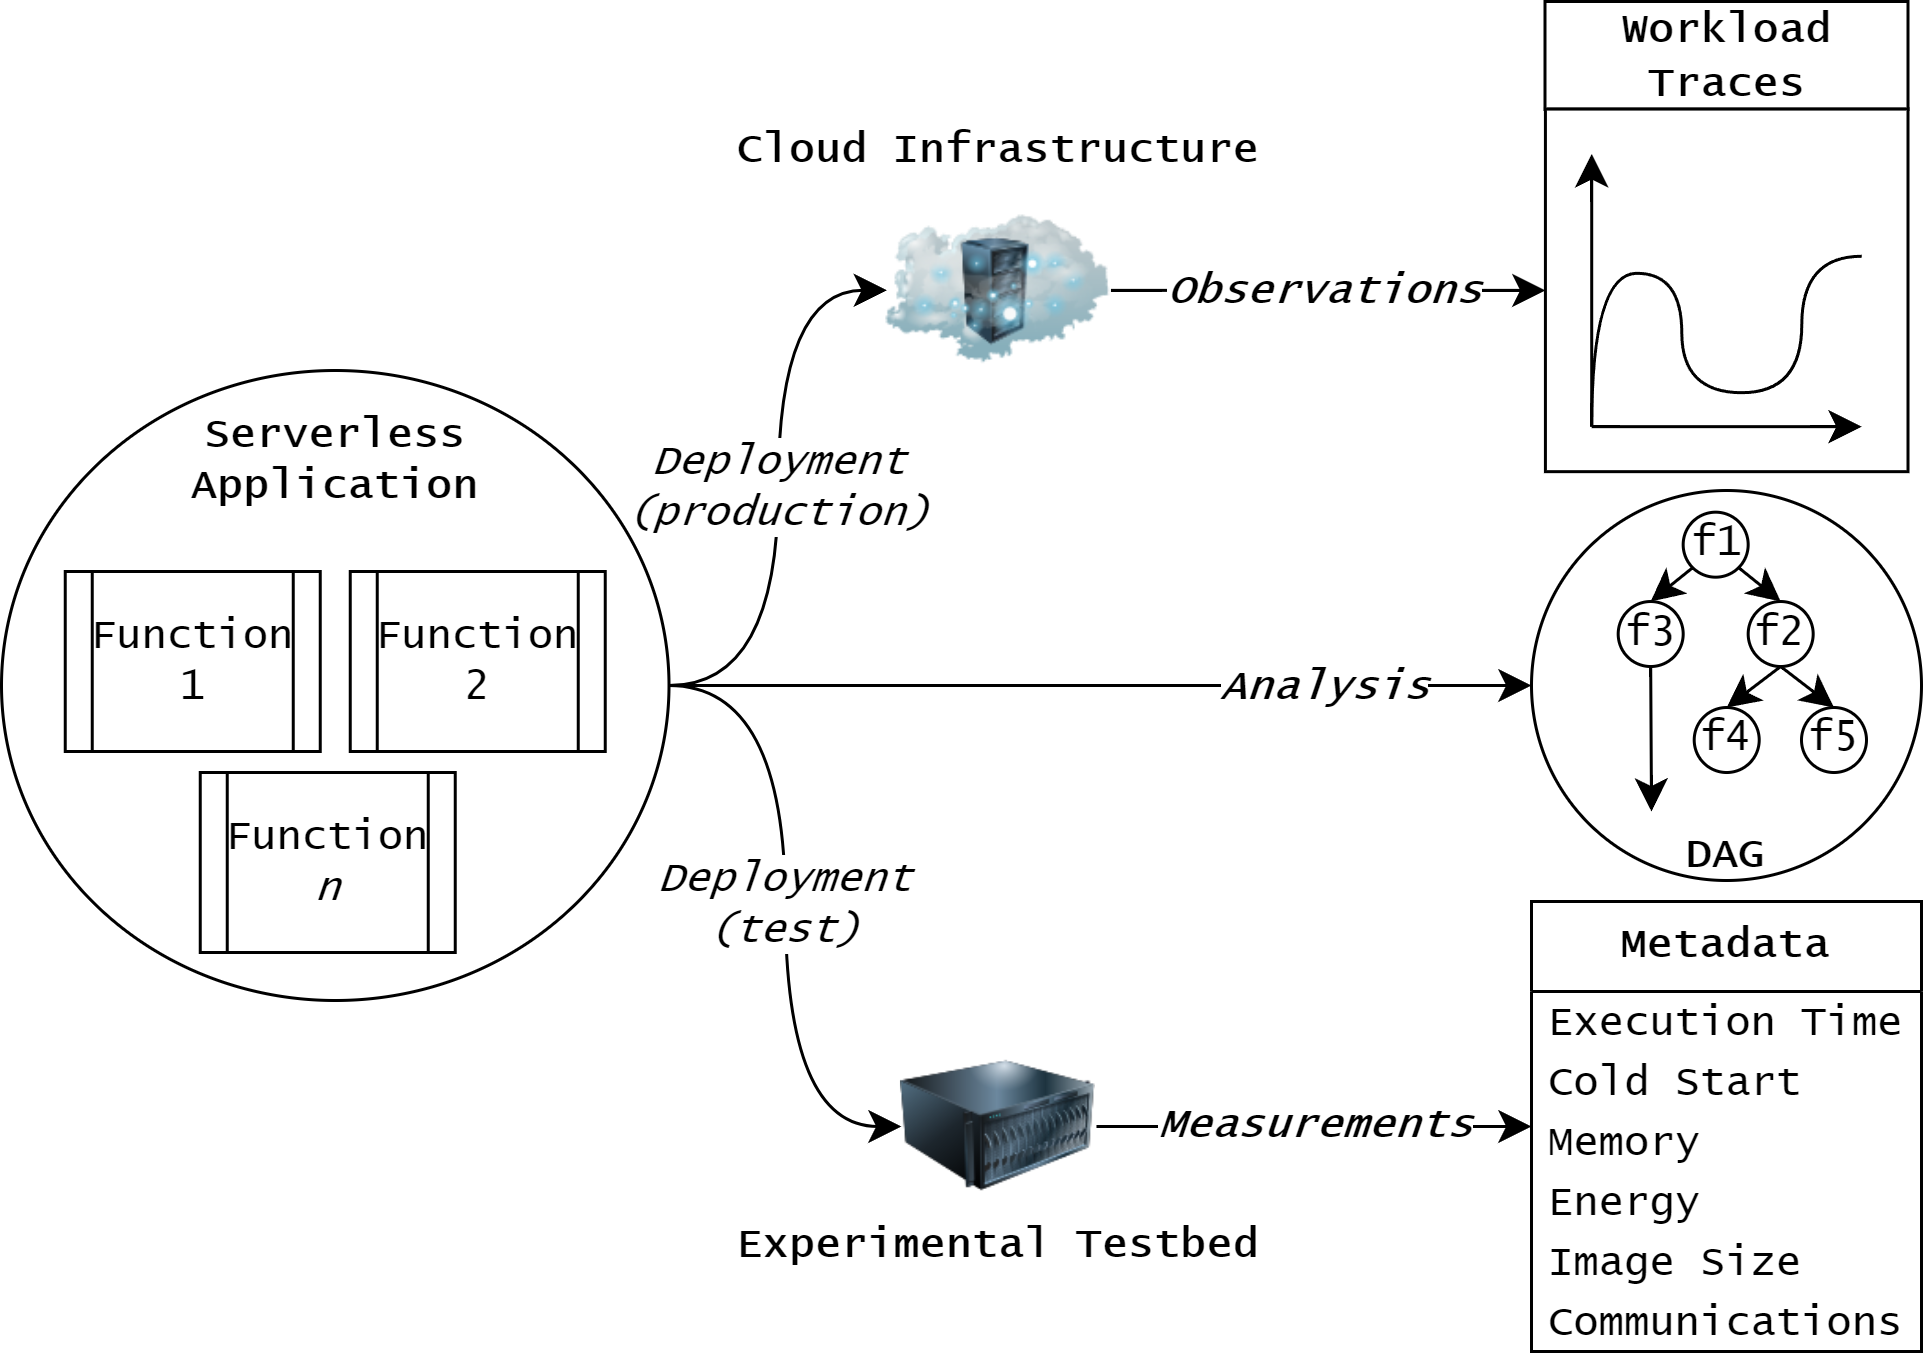
\includegraphics[width=0.7\textwidth]{6_Chapitre6/figures/characterization.png}
    \caption{Une vue d'ensemble de notre méthodologie de caractérisation.}
\label{figure:herosim-characterization}
\end{figure}

Pendant la simulation, des journaux sont écrits sur le disque. Lorsque toutes les requêtes de la trace d'exécution ont été traitées, la simulation s'arrête et retourne les résultats ainsi que des graphiques résumant la simulation, respectivement dans les répertoires \texttt{result} et \texttt{chart}.

Le simulateur est monotâche, ce qui signifie que chaque politique est évaluée de manière séquentielle, au cours d'une exécution complète du scénario. Cependant, plusieurs instances de HeROsim peuvent être exécutées en parallèle, avec différentes configurations, sur plusieurs cœurs de \gls{CPU}, voire même distribuées sur plusieurs nœuds. Chaque instance de HeROsim exécutant une politique d'orchestration différente et toutes les instances utilisant un répertoire de sortie commun, il est possible d'accélérer la durée totale de la simulation lors de l'évaluation de nombreuses politiques d'orchestration. Lorsque toutes les exécutions du simulateur sont terminées, les résultats consolidés peuvent être passés au module d'analyse et de génération des graphiques.

\subsection{Module Orchestrateur}

Le rôle principal du module d'orchestrateur est de maintenir une vue sur l'état du système qui sera utile à l'autoscaler et à l'ordonnanceur. La classe de base \textbf{\texttt{Orchestrator}} fournit des méthodes d'initialisation abstraites qui doivent être redéfinies pour spécifier la structure de données à l'état du système que l'on souhaite modéliser et l'initialiser. Par exemple, un ordonnanceur \textit{Round Robin} devra savoir combien de fois chaque réplique de fonction est sélectionnée pour le placement des tâches, tandis qu'un ordonnanceur \textit{Least Connected} devra connaître la concurrence moyenne dans chaque réplique pour équilibrer la charge. Cette classe est le point d'entrée permettant aux utilisateurs de définir des méthodes qui seront appelées pendant la simulation, périodiquement ou à la suite d'un évènement, et permettront de maintenir à jour un ensemble de métriques qui représente de manière pertinente l'état de la plateforme à tout instant.

Les utilisateurs peuvent mettre en œuvre des processus périodiques de gestion de l'état du système en fonction de leurs besoins pour supporter une variété de politiques d'orchestration. L'orchestrateur de base est doté d'un système simple qui peut fonctionner tel quel ou être étendu. Dans notre implantation, un processus de surveillance est appelé périodiquement pour garder une trace de la concurrence moyenne dans chaque réplique de fonction. Ceci est utile pour les politiques basées sur des seuils, telles que présentées dans les chapitres~\ref{chapter:herofake} et~\ref{chapter:herocache}.

La méthode du point d'entrée de l'orchestrateur est appelée chaque fois qu'une requête utilisateur arrive sur la plateforme. Elle prend en entrée l'état du système et la requête utilisateur. Elle peut être redéfinie dans chaque implantation de politique d'orchestration pour permettre une mise à l'échelle automatique et une ordonnanceur à grain fin, selon les besoins.

Enfin, cette classe est responsable de l'instanciation des implantations sélectionnées pour l'\texttt{Autoscaler} et le \texttt{Scheduler}. Toute combinaison de ces deux modules peut être instanciée par l'orchestrateur.

\subsection{Module Autoscaler}

La classe de base \textbf{\texttt{Autoscaler}} fournit le comportement commun de la plateforme d'autoscaling, qui correspond essentiellement au cycle de vie des répliques de fonctions, de leur création à leur suppression. Plusieurs méthodes abstraites doivent être redéfinies pour mettre en œuvre une nouvelle politique : stratégie de sélection des ressources pour la création de répliques, processus d'initialisation des répliques, sélection des répliques pour la suppression, etc. Ces méthodes opèrent à la granularité d'une seule fonction, en prenant l'état du système et la liste des ressources matérielles disponibles comme données d'entrée. Les utilisateurs sont libres de mettre en œuvre les algorithmes qu'ils souhaitent évaluer pour la gestion des ressources.

L'autoscaler de HeROsim a été principalement conçu pour une \textbf{mise à l'échelle horizontale}. Les répliques de fonctions sont créées en allouant une plateforme d'exécution et la quantité requise de mémoire sur un nœud. Une plateforme d'exécution ne peut pas héberger plus d'une réplique de fonction à la fois. Pour faire face à l'augmentation de la charge d'une application sans dégradation de la qualité de service, de nouvelles répliques de fonctions doivent être allouées par l'autoscaler, à condition qu'il y ait suffisamment de ressources matérielles disponibles. Les répliques nouvellement allouées passent par une phase d'initialisation au cours de laquelle les images des fonctions doivent être récupérées via le réseau. L'autoscaler peut gérer un cache d'images dans la mémoire du nœud et sur le stockage local du nœud afin d'accélérer les démarrages à froid.

La suppression des répliques inactives se fait sur le mode \textit{best effort} : l'autoscaler tente de supprimer les répliques dont les files d'attente de tâches sont vides. Par défaut, une réplique avec des tâches en attente ne peut pas être supprimée. Ce comportement pourrait être redéfini par une nouvelle politique, qui par exemple prendrait en charge les migrations de tâches.

L'autoscaler garde une trace de chaque événement d'allocation pour calculer l'utilisation des ressources à la fin de la simulation. HeROsim permet à l'utilisateur de savoir quels nœuds et quelles plateformes d'exécution ont été enrôlés pendant le scénario, à quel moment et pour quelle durée, et pour quel déploiement de fonction ils ont été choisis. Cela permet également à HeROsim de calculer la consommation d'énergie à différentes granularités : la consommation statique nécessaire au matériel alloué, et la consommation dynamique liée à l'exécution des applications.

% TODO: modèle énergétique, modèle temporel

HeROsim est livré avec les politiques de mise à l'échelle automatique suivantes, basées sur des seuils de concurrence et prêtes à l'emploi :

\begin{itemize}
    \item \textit{Random} -- Sélectionne un nœud aléatoire et une plateforme d'exécution pour les nouvelles répliques ;
    \item Knative -- Sélectionne le nœud le moins chargé pour allouer de nouvelles répliques, \textit{i.e} équilibre les charges de travail sur un grand nombre de nœuds ;
    \item HeROfake (voir chapitre~\ref{chapter:herofake}) -- Exploite l'hétérogénéité du matériel pour minimiser les pénalités de qualité de service, la consommation d'énergie et le coût total de possession. Plus de détails sont donnés dans la section~\ref{section:herosim-case-study};
    \item HeROcache (voir chapitre~\ref{chapter:herocache}) -- Optimise les allocations pour les chaînes de fonctions ; maximise la consolidation des fonctions de chaque application. Plus de détails sont donnés dans la section~\ref{section:herosim-case-study}.
\end{itemize}

\subsection{Module Ordonnanceur}

La classe de base \textbf{\texttt{Scheduler}} met en œuvre la sélection des tâches dans la file d'attente de la plateforme. Une méthode abstraite doit être redéfinie pour mettre en œuvre une nouvelle politique : la sélection d'une réplique parmi le pool de répliques disponibles, pour placer chaque requête utilisateur en attente. Cette méthode opère à la granularité la plus fine : elle est appelée lors de la réception d'une requête, et prend en entrée l'état du système et la liste des répliques de fonctions disponibles.

Les requêtes utilisateur arrivent dans une file d'attente au niveau de l'ordonnanceur. Les utilisateurs peuvent mettre en œuvre leur propre politique de priorité pour la sélection des tâches ou choisir une politique déjà disponible dans le simulateur, \textit{e.g.} \textit{First In, First Out} (\gls{FIFO}) ou \textit{Earliest Deadline First} (\gls{EDF})~\cite{herofake}.

L'ordonnanceur de HeROsim a été conçu sans tenir compte des défaillances ou des migrations de tâches : le comportement par défaut considère des tâches qui s'exécutent toujours avec succès jusqu'à leur terme. Cependant, les tâches seront marquées comme "en pénalité" si l'ordonnanceur manque leur échéance. Cette valeur booléenne permet d'évaluer la qualité de politiques d'orchestration en matière de respect des exigences de qualité de service : elle indique la proportion de requêtes qui ne sont traitées en temps voulu.

S'il n'y a pas de réplique disponible au moment de l'ordonnancement d'une requête utilisateur, l'ordonnanceur fera un appel à l'autoscaler pour forcer la création d'une première réplique pour la fonction. Dans l'intervalle, la requête est remise dans la file d'attente et reportée. Les tâches reportées sont signalées comme telles, de sorte que, par exemple, elles puissent avoir une priorité plus élevée si toutefois l'utilisateur souhaite appliquer une telle politique~\cite{herocache}.

HeROsim est livré avec les politiques d'ordonnancement suivantes implantées et prêtes à l'emploi :

\begin{itemize}
    \item \textit{Random} -- Sélectionne une réplique aléatoire pour le placement des tâches ;
    \item Knative -- Sélectionne la réplique avec la file d'attente la plus courte pour le placement des tâches ;
    \item \gls{BPFF} -- Sélectionne la réplique avec la plus longue file de requêtes en attente pour le placement des tâches ;
    \item HeROfake (voir chapitre~\ref{chapter:herofake}) -- Sélectionne la réplique qui minimise un score calculé en fonction de l'échéance de la tâche, de la consommation d'énergie de la fonction et de la dispersion des tâches sur les nœuds. Plus de détails sont donnés dans la section~\ref{section:herosim-case-study} ;
    \item HeROcache (voir chapitre~\ref{chapter:herocache}) -- Sélectionne la réplique d'une manière similaire à HeROfake, mais prend en compte les opérations de stockage et de communication pour calculer la latence de bout en bout de la requête, et prend en compte les chaînes de fonctions lors du calcul du score des répliques en ce qui concerne la consolidation des tâches. De plus amples détails sont donnés dans la section~\ref{section:herosim-case-study}.
\end{itemize}

\subsection{Interface utilisateur}

HeROsim s'appuie sur des journaux d'évènements pour fournir un aperçu du déroulement de la simulation, ce qui aide l'utilisateur à déboguer ses politiques. À la fin de la simulation, des fichiers de résultats sont enregistrés sur le disque. Ces fichiers contiennent un résumé des résultats de la simulation, c'est-à-dire les performances de la politique au regard des métriques d'évaluation (qualité de service, consommation d'énergie, etc.). Ces résultats sont représentés sur différents graphiques qui peuvent être utilisés dans des publications ultérieures (voir chapitres~\ref{chapter:herofake} et~\ref{chapter:herocache}).

HeROsim peut également générer des graphiques supplémentaires, utiles pour tracer le comportement de la plateforme lors de l'élaboration d'une politique d'orchestration. On peut ainsi visualiser la proportion de démarrages à froid et d'accès au cache parmi les invocations de fonctions. HeROsim peut également tracer la latence par quantiles pour les requêtes des utilisateurs, ce qui peut aider à identifier un éventuel problème de dimensionnement d'une infrastructure cloud. Le générateur de traces d'exécution trace les temps d'arrivée des requêtes utilisateur, ce qui permet de visualiser sur un graphique les caractéristiques de la charge de travail.

\begin{figure}[!ht]
    \centering
    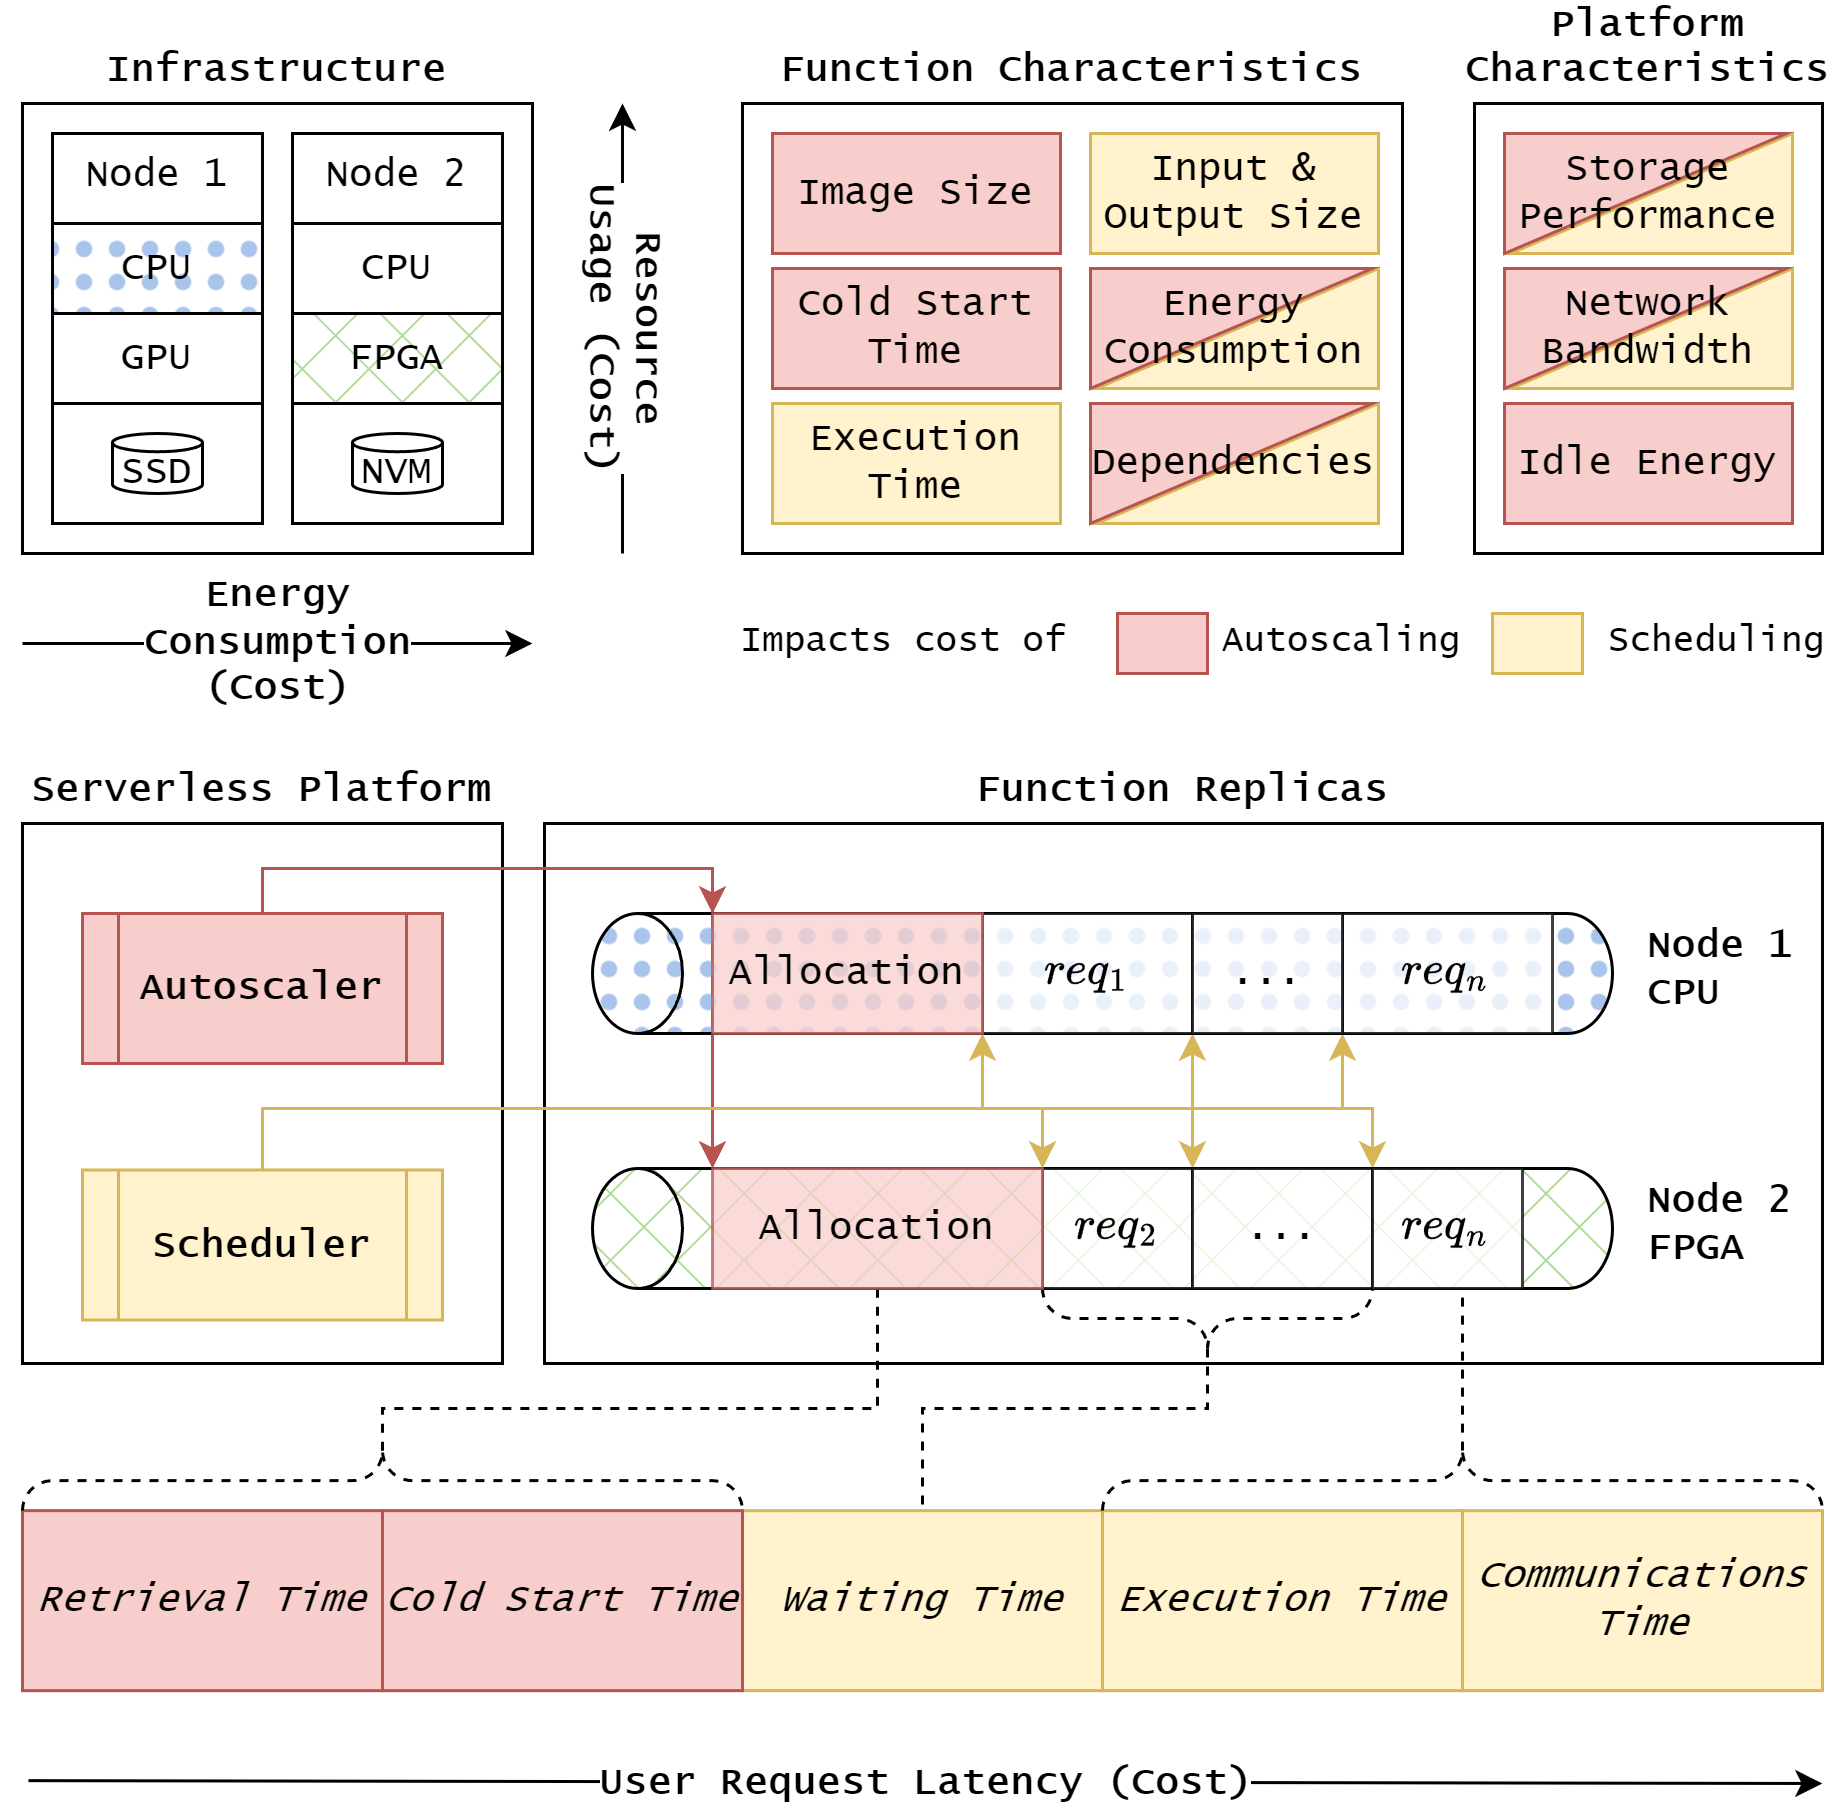
\includegraphics[width=0.7\textwidth]{6_Chapitre6/figures/serverless-cost.png}
    \caption{Répartition du coût en latence de bout en bout induit par les décisions d'autoscaling et d'ordonnancement.}
\label{figure:herosim-cost}
\end{figure}

\section{Étude de cas}
\label{section:herosim-case-study}

% TODO: Figures de développement (tail latency, etc.) ?

Dans cette section, nous présentons deux études de cas dans le cadre desquelles HeROsim a permis de concevoir et d'évaluer différentes politiques d'orchestration serverless. Nous avons conçu des stratégies qui reposent sur la caractérisation de plateformes hétérogènes et des charges de travail à déployer (voir figure~\ref{figure:herosim-characterization}). Nous avons mesuré plusieurs métriques liées à nos applications sur diverses plateformes matérielles et proposé un modèle de coût qui intègre ces valeurs, dans le but d'estimer les performances de l'autoscaler et de l'ordonnanceur sous différentes politiques (figure~\ref{figure:herosim-cost}).

\subsection{Stratégie d'orchestration de fonctions sans état sur ressources hétérogènes}

Dans cette première étude de cas, HeROfake (pour \textbf{He}terogeneous \textbf{R}esources \textbf{O}rchestration for deep\textbf{fake} detection~\cite{herofake}) (voir chapitre~\ref{chapter:herofake}), nous avons étudié le déploiement d'une application de détection de deepfake sur une plateforme serverless dans un cloud privé. En particulier, nous nous sommes intéressés à l'exploitation de ressources hétérogènes pour l'orchestration serverless lors de l'optimisation de la plateforme pour la \gls{QoS} et la consommation d'énergie.

L'application exécute des tâches d'inférence pour détecter des deepfakes dans des images soumises par des utilisateurs avec diverses exigences de niveau de \gls{QoS}. Son objectif est de détecter les images potentiellement falsifiées, c'est-à-dire les images susceptibles d'avoir été manipulées par ordinateur pour tromper des spectateurs ou destinataires. Elle se compose de trois fonctions, basées sur l'utilisation de réseaux de neurones, indépendantes et sans état, qui ont été mises en œuvre sur du matériel hétérogène : \gls{CPU}, \gls{GPU} et \gls{FPGA}. Ces implantations ont été utilisées pour les mesures, mais il aurait été difficile d'exécuter des scénarios réalistes sur une plateforme serverless prenant en charge ces architectures matérielles. Ainsi, nous avons eu recours à la simulation pour estimer les performances de notre stratégie d'orchestration.

Dans HeROfake, chaque exécution de tâche a un coût associé mesuré en \textbf{latence}. L'allocation de nouvelles répliques sur des ressources matérielles inactives introduit un \textbf{délai de démarrage à froid} ; le traitement des requêtes utilisateur sur différentes architectures matérielles donne lieu à des variations en matière de \textbf{temps d'exécution de la fonction}. La latence de chaque requête utilisateur est finalement comparée à l'\textbf{exigence de qualité de service} de la requête : si l'échéance de la requête n'a pas été respectée, la tâche est en \textbf{pénalité}. Ces éléments constituent la base de notre modèle de coût, comme illustré dans la figure~\ref{figure:herosim-cost}.

Les différentes architectures matérielles ont également des coûts monétaires et énergétiques différents qui ont été pris en compte dans le modèle de coût (utilisation des ressources et consommation d'énergie, les deux dimensions du coût de l'infrastructure montré dans la figure~\ref{figure:herosim-cost}). Nous avons mis en œuvre un autoscaler et un ordonnanceur qui cherchent à estimer et à minimiser ce coût composite, à la granularité de chaque requête utilisateur. L'autoscaler cherche à allouer des plateformes qui minimisent le coût global, y compris l'utilisation des ressources, la consommation d'énergie et le coût total de possession. L'ordonnanceur cherche à sélectionner les répliques qui traitent les requêtes avec le moins de pénalités et la plus faible consommation d'énergie.

HeROfake a été évalué pour un scénario synthétique avec une distribution uniforme des temps d'arrivée des requêtes, des types de fonction appelées et des niveaux de qualité de service associés aux requêtes. HeROfake s'est avéré performant (en termes de pénalités sur \gls{QoS}, de consolidation des tâches et d'énergie consommée) par rapport à Knative (l'orchestrateur serverless de Google) et \textit{Bin-Packing First Fit} (\gls{BPFF}, la politique d'\gls{AWS} pour Lambda)~\cite{herofake}.

Notre objectif principal était d'étudier la pertinence de la prise en compte de l'hétérogénéité matérielle lors de l'allocation des ressources et de l'ordonnancement des requêtes utilisateur au regard de différentes mesures de qualité de service, \textit{i.e.} la latence de bout en bout subie par les requêtes utilisateur, et la consommation d'énergie de l'infrastructure. Les résultats expérimentaux ont montré que si le temps total d'exécution des tâches dans HeROfake est similaire à celui de Knative, nous obtenons une réduction de plus de 60\% des pénalités sur qualité de service ; les tâches sont consolidées sur moins de 40\% des nœuds de l'infrastructure, 77\% des plateformes d'exécution restant inutilisées ; et la consommation d'énergie dynamique est réduite de 35\% par rapport à Knative.

HeROsim nous a également permis d'évaluer l'impact des différents composants de notre orchestrateur. Les résultats ont montré que, même en allouant uniquement des \gls{CPU}, l'ordonnancement des requêtes avec notre politique consciente de la qualité de service pouvait maintenir les pénalités en dessous de 50\%.

\subsection{Stratégie d'orchestration d'applications avec prise en compte du cache et des communications}

Dans une seconde étude, nous avons conçu un orchestrateur pour les applications serverless, composées de plusieurs fonctions interdépendantes. Nous avons proposé HeROcache (pour \textbf{He}terogeneous \textbf{R}esources \textbf{O}rchestration with a \textbf{cache} strategy~\cite{herocache}) (voir chapitre~\ref{chapter:herocache}), une stratégie d'orchestration consciente des contraintes temporelles et de données. Nous avons exploré le déploiement d'un système de détection d'intrusion (\gls{IDS}, pour \textit{Intrusion Detection System}) sur une plateforme serverless. En particulier, nous avons étudié les avantages de l'orchestration consciente des données lors de l'exploitation de matériel hétérogène pour déployer des applications sensibles au temps sur des dispositifs \textit{edge} à ressources limitées, du point de vue du fournisseur de services.

L'objectif de l'application est de détecter le trafic réseau potentiellement malveillant dans des journaux soumis par les utilisateurs.
% Comme cette application d'\gls{IDS} est spécifiquement destinée aux missions de drones, la fréquence des requêtes utilisateur présente une saisonnalité, ce qui en fait un bon cas d'étude pour le paradigme serverless : les ressources matérielles pourront être libérées lorsque l'application n'est pas utilisée.
L'application se compose de deux couches pour traiter les requêtes utilisateur : deux fonctions de prétraitement, qui opèrent sur les journaux de trafic réseau pour exclure les évènements que l'on sait légitimes, et quatre fonctions d'inférence, basées sur des réseaux de neurones entraînés à détecter des motifs typiques d'activité malveillante dans le reste des journaux. Ces fonctions ont été mises en œuvre sur différentes architectures matérielles (\gls{CPU}, \gls{FPGA}, \gls{GPU}).

Il existe des dépendances de données entre les deux couches de l'application. Nous les avons modélisées sous forme de graphes acycliques dirigés (\gls{DAG}) d'appels de fonctions. Nous avons utilisé le module Python \texttt{TopologicalSorter} du module \texttt{graphlib} pour lire et écrire la représentation \gls{JSON} des graphes et pour les parcourir pendant l'exécution.

Au niveau de l'orchestrateur, nous avons dû modifier la granularité des requêtes utilisateur : dans HeROcache, une requête concerne une application, qui peut être composée d'une ou plusieurs fonctions, appelées dans l'ordre défini par le \gls{DAG} de l'application. Chaque fonction peut prendre des données en entrée et produire des données en sortie. Ces données sont définies par leur taille en octets.

Alors que HeROfake ne prend pas en compte les coûts associés opérations de stockage, HeROcache considère la \textbf{récupération des images de fonctions}, la \textbf{mise en cache des images de fonctions} et les \textbf{communications entre fonctions} dans les décisions de l'autoscaler et de l'ordonnanceur. Nous avons étendu HeROsim avec ces concepts pendant la conception de HeROcache. Ces opérations impactent la latence des requêtes utilisateur. Des mesures hors-ligne pour caractériser les fonctions permettent à HeROsim, comme montré dans la figure~\ref{figure:herosim-cost} d'estimer le temps de récupération de l'image de la fonction sur la base du débit du lien réseau spécifié par l'utilisateur dans la description de l'infrastructure, la taille de l'image de la fonction spécifiée par le type de charge de travail, et la performance du stockage local au nœud spécifiée par le type de stockage.

L'introduction d'opérations de stockage à la granularité d'un nœud nous a permis d'évaluer une stratégie de préchargement des images de fonctions au sein d'une application, qui peut accélérer les démarrages à froid pour des invocations futures.

Dans HeROcache, l'autoscaler cherche à accroître la consolidation des fonctions entre les applications, à réduire la durée de réalisation globale (ou \textit{makespan}), la consommation d'énergie et le coût total de possession. L'ordonnanceur cherche à éviter la violation des échéances des requêtes, à consommer moins d'énergie et à assurer une utilisation élevée des ressources mobilisées.

HeROfake est conçue comme une politique sans conscience du stockage, mais exploite déjà l'hétérogénéité matérielle, ce qui en fait une solution comparable. Cette comparaison nous a permis de montrer l'importance de la prise en compte des coûts de stockage dans la capacité de la plateforme à respecter les exigences de qualité de service : en prenant compte de ces coûts, HeROcache consolide les applications et parvient à réduire les délais d'initialisation moyens de 17,6\% et les délais de communication de 88,4\%. Cela permet de réduire la consommation d'énergie statique de la plateforme de 80\% tout en maintenant moins de 28\% de violations de qualité de service.

HeROcache (mis en œuvre dans HeROsim) a été soumis pour évaluation des artefacts et a reçu les trois badges de reproductibilité de l'IEEE~\footnote{\href{https://www.niso.org/standards-committees/reproducibility-badging}{https://www.niso.org/standards-committees/reproducibility-badging}} lors de sa publication : \textit{Open Research Objects} (ORO), \textit{Reusable/Research Objects Reviewed} (ROR), et \textit{Results Reproduced} (ROR-R).

% \section{Travaux connexes}
% \label{section:herosim-sota}

% Nous présentons un aperçu des travaux de l'état de l'art en matière de simulation pour le cloud, et proposons une comparaison d'un ensemble de leurs caractéristiques dans le tableau~\ref{table:herosim-sota}.

% CloudSim~\cite{calheiros_cloudsim_2011} est l'outil de référence pour les expériences de déploiement cloud à grande échelle. Il cible les différents modèles de service traditionnels dans le cloud (\gls{IaaS}, \gls{PaaS}, \gls{SaaS} ; voir chapitre~\ref{chapter:context}).
% CloudSim et ses extensions~\cite{calheiros_cloudsim_2011, mampage_cloudsimsc_2023, wickremasinghe_cloudanalyst_2010, jeonCloudSimExtensionSimulatingDistributed2019} ne prennent pas en compte les applications serverless, \textit{i.e.} la composition de fonctions pour décrire un comportement complexe qui introduit des défis spécifiques (délais de démarrage à froid, coûts liés aux communications inter-fonctions, etc.~\cite{wawrzoniakBoxerDataAnalytics2021a}).
% Pour relever ces défis en simulation, il est nécessaire d'introduire la gestion du stockage, ainsi que le traitement des chaînes de fonctions, comme le fait HeROsim.

% DFaaSCloud~\cite{jeonCloudSimExtensionSimulatingDistributed2019} est un autre simulateur basé sur CloudSim pour le serverless distribué. Ce travail se concentre sur la distribution géographique des instances de fonction à travers une infrastructure cloud, edge et fog. Il permet d'estimer les retards induits par la localité des fonctions. Les utilisateurs définissent la qualité de service pour leurs fonctions en termes de contraintes de latence et DFaaSCloud fournit une politique de placement qui minimise les violations et les coûts. Nous n'avons pas abordé la dimension géographique du problème de placement dans les travaux de cette thèse.

% ElasticSim~\cite{cai_elasticsim_2017} étend également CloudSim pour fournir une allocation dynamique des ressources pour \textit{workflows} dans le cloud, \textit{i.e.} des chaînes de tâches interdépendantes, qui présentent des similitudes avec les applications serverless. Cependant, il ne prend pas en compte l'hétérogénéité des ressources matérielles et ne permet pas non plus d'appliquer des objectifs de qualité de service par requête. OpenDC 2.0~\cite{mastenbroekOpenDCConvenientModeling2021} est un outil généraliste et très complet qui autorise également l'utilisateur à modéliser de telles chaînes de fonctions. Bien que cet outil permette de représenter un centre de données hétérogène et d'estimer sa consommation d'énergie, il ne prend pas non plus en compte la variété des exigences des utilisateurs en termes de latence.

% GridSim~\cite{buyyaGridSimToolkitModeling2002} présente des caractéristiques intéressantes, allant de la modélisation d'infrastructures hautement hétérogènes à la prise en charge de contraintes de qualité de service par requête. Cependant, il se concentre sur des infrastructures dites "en grille", que l'on trouve généralement dans le monde du calcul haute performance (\gls{HPC}, pour \textit{High Performance Computing}), et ne permet pas d'explorer des problèmes liés à l'allocation dynamique de ressources. iFogSim2~\cite{mahmudIFogSim2ExtendedIFogSim2021} considère également des allocations statiques qui ne peuvent pas caractériser fidèlement l'espace de problème serverless.
% HeROsim a été conçu pour le serverless et permet aux utilisateurs de tracer les événements d'allocation et d'ordonnancement à la granularité d'une requête utilisateur.

% De nombreuses contributions~\cite{jeonCloudSimExtensionSimulatingDistributed2019, cai_elasticsim_2017, buyyaGridSimToolkitModeling2002, nunez_icancloud_2012} ne permettent pas d'estimer la consommation d'énergie de la plateforme. La consommation d'énergie est une mesure cruciale lorsqu'il s'agit de relever le défi de l'ordonnancement de calculs gourmands en énergie tels que l'apprentissage automatique (\gls{ML}), qui représentent une proportion croissante des charges de travail déployées dans le cloud~\cite{masanetRecalibratingGlobalData2020}.
% HeROsim estime à la fois la consommation d'énergie statique et la consommation d'énergie dynamique.

% En outre, l'hétérogénéité du matériel est une caractéristique déterminante du cloud. Les accélérateurs tels que les \gls{GPU} ou les \gls{TPU} sont utilisés par les fournisseurs de services pour améliorer la performance de charges de travail adaptées, bénéficiant largement de ces architectures matérielles. Nous avons soutenu qu'exploiter ce matériel de manière opportuniste pourrait permettre aux fournisseurs de services de proposer des accords de niveau de service pour le cloud serverless, tout en réduisant la consommation d'énergie de leur plateforme~\cite{herofake}.
% Parmi les outils de simulation disponibles pour le cloud, plusieurs contributions~\cite{jeonCloudSimExtensionSimulatingDistributed2019, cai_elasticsim_2017, nunez_icancloud_2012, mahmoudiSimFaaSPerformanceSimulator2021} ne prennent pas en compte l'hétérogénéité à une granularité fine. HeROsim permet aux utilisateurs de définir des infrastructures hautement hétérogènes, à la fois pour le calcul et pour le stockage.

% Enfin, certaines contributions~\cite{nunez_icancloud_2012, mahmoudiSimFaaSPerformanceSimulator2021} visent à simuler des infrastructures de cloud public et se concentrent sur la réservation de ressources virtualisées considérées comme illimitées, utilisées par exemple dans le cadre d'un panachage, pour répartir les charges de travail entre un cloud privé et un cloud public dans le but de diminuer les coûts.
% Nos travaux~\cite{herofake, herocache} se sont concentrés sur la perspective de fournisseurs de services optimisant leurs plateformes serverless pour la qualité de service, d'où l'orientation cloud privé de HeROsim.

\section{Conclusion et perspectives}
\label{section:herosim-conclusion}

Dans cet article, nous avons présenté HeROsim, un outil de simulation qui vise à permettre aux chercheurs de modéliser des infrastructures cloud hétérogènes, de décrire des charges de travail à une granularité fine, de mettre en œuvre diverses politiques de gestion des ressources et d'ordonnancement des tâches, et d'évaluer leur efficacité au regard de métriques telles que l'utilisation des ressources, la consommation d'énergie, les violations de la QoS par requête, ou la latence des files d'attente. HeROsim peut générer des graphiques qui aident à visualiser ces résultats pendant la phase de mise en œuvre et peuvent être utilisés dans des publications.

Des travaux sont en cours pour étendre HeROsim et proposer une interface web permettant de visualiser l'état de la simulation en temps réel. Nous travaillons également sur un agent d'apprentissage par renforcement qui pourrait être inclus dans une prochaine version.
